A physical fitness test usually evaluates multiple components of one's health, including cardiovascular endurance, muscular strength, muscular endurance, flexibility and body composition.

In this chapter I will focus on familiarizing the reader with cardiovascular endurance testing, as it has the largest effect on hiking.
There is a number of indicators that one can measure (such as the lactate threshold - a non-linear increase in blood lactate concentration\cite{lactate-threshold}), 
but the most popular and easiest to measure with a heart rate monitor is VO2 max.

\section{VO2 and VO2 max}

The volume of consumed oxygen (VO2) is closely correlated with heart rate, respiration rate, and on/off-dynamics, all of which can be derived from RR interval data (time elapsed between two sucessive R waves -- the tallest spikes on an ECG),
with respiration rate being able to differentiate between metabolic (physical acitivity induced) and non-metabolic (mental and non-exercise related physical stress) changes in heart rate,
which makes models that take it into account highly accurate compared to those which only use heart rate.\cite{vo2-hr-firstbeat}

VO2 max, the maximal value of VO2, is considered the most accurate metric of cardiovascular fitness.

Measured in millilitres of oxygen consumed per minute or millilitres of oxygen per kilogram of bodyweight per minute, it is the amount of oxygen the body is able to effectively use (transform to energy) during intense or maximal exercise.
With the growing amount of oxygen the body can consume, it can perform better during strenuous activity and give improved results.\cite{vo2max-definition}
This is limited by the ability of the cardiorespiratory system to deliver oxygen to the exercising muscle, thus making it impossible for an athlete to operate above 100\% of their VO2 max for extended periods.\cite{vo2max-oxygen-delivery}

\begin{figure}[h]
    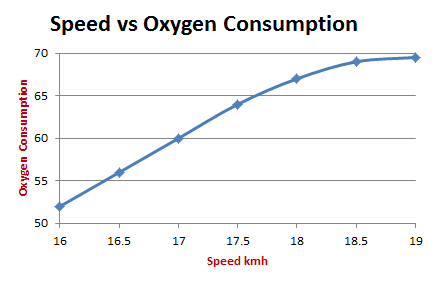
\includegraphics[width=\textwidth]{V02max-running.png}
    \caption{With increasing speed, oxygen consumption increases linearly and plateaus around 18.5 kilometres per hour \cite{vo2max-speed-img}}
\end{figure}

\subsection{How to measure Vo2 max}

\subsubsection*{Laboratory test}

Typically, VO2 max is measured directly in laboratory conditions while wearing a respiratory mask, by analyzing inspired and expired breathing gases during maximal exertion,\cite{vo2max-definition} usually running on a treadmill.
This method of determining VO2 max is highly accurate, but given the need for expensive equipment and trained staff, laboratory testing just isn't feasible for everyday population-wide testing.

\subsubsection*{Cooper test - Twelve-Minute Run-Walk}

First suggested in the 1970's, Cooper's Twelve-Minute Run-Walk is an endurance test, where the main goal is to run (or walk) as long a distance as possible in twelve minutes.
It was originally developed mainly for armies and police agencies, but it's also popularly (and unnecessarily\cite{cooper-pupils}) used in schools on untrained pupils.
It may also be inaccurate for people who do not train running and swim or bike instead, as their bodies are used to a completely different set of movements.

There is a high correlation between the distance an individual can run and their VO2 max value, which can be calculated thusly:

$VO2max = (22.351 \times distance_in_kilometers) - 11.288$\cite{cooper-vo2max}

\subsubsection*{Multistage Fitness Test - Beep test}

Introduced by a Canadian sport scientist Luc Léger in the 1970's, this aerobic test has consistently been found a reliable way of finding a person's VO2 max.

The original version of the beep test (the Track Test) had the participants running back and forth in the interval of two minutes while the running pace was increased, so they always had to run further than in the previous iteration.

This test was highly efficient, however, given the long intervals and spatial requirements, it couldn't be performed indoors, giving rise to modifications, such as the Twenty-Metre Shuttle Run Test.
As the name suggests, two markers are placed twenty metres apart and again, the participants run back and forth between them, trying to reach the opposite marker before the next -- shorter -- stage begins, that is, before the next beep.
Once the test subject fails to reach a marker, turns without touching the marked line, or starts running before the signal, after one warning, their test is over.
They can also choose to stop when they have reached their maximum physical limit.

The test is divided into stages with recommended running speeds, each stage consisting of multiple shuttles - see the table at \cite{beep-test-scoring-table}.
From the stage and shuttle reached, one can calculate the VO2 max using the formula

\[VO2max (\frac{ml}{kg*min-1}) = 31.025 + 3.238X - 3.248A + 0.1536AX\],

where A is age of the participant and X is the speed in the final shuttle.
This formula fits the commonly used version of the Beep test (starting at 8.0 km/h, jumping to 9.0 km/h and continuing to rise by 0.5 km/h per level) and may vary depending on the version used.\cite{beep-test-versions}\cite{beep-test-20m-valid}

This modified version (just like the original) has been recognized as a valid method to determine VO2 max of male and female adults, individually or in groups, on most gymnasium surfaces.\cite{beep-test-20m-valid}

In 2017, Tomkinson et al. published a complex systematic study of nearly 1.2 million 9-17 years old children from 50 countries with data from beep tests as old as 1981,
setting standardized norms for testing of fitness in the world's youth.\cite{beep-test-youth-large-study}


\subsubsection*{Walking tests}

\section{The Performance Condition}

A person's VO2 max is recognized as their baseline fitness level index, however, everybody has days when they perform better, and days when they perform worse, while the factors in play are the amount of sleep they get, being sore from previous workouts, and general physical and mental wellbeing.

That is why Firstbeat introduced the Performance Condition.

Firstbeat is a provider of physiological analytics for sports and well-being who have translated human physiology into mathematical models based on heart rate variability (see below).
They provide their analytics engine as a service to a number of fitness device manufacturers, such as Garmin, Xiaomi, Honor and others.

The Performance Condition is a real-time index of a user's immediate fitness and fatigue level compared to their baseline fitness level.

This indicator is measured on a scale of -20 to +20, with each point representing roughly 1\% of their Vo2 max.
So if the user's current Performance Condition is +4, they can expect to perform outstandingly,
but at the same time, during the course of a workout, this number will decrease as fatigue from the exercise gets closer.\cite{performance-condition-firstbeat}\cite{performance-condition-garmin}

According to Firstbeat's support personnel, the formula behind the Performance Condition is protected information,
but generally, it uses a combination of personal background information, internal and external workload data, and special guidance from the Firstbeat analytics engine.\cite{firstbeat-performance-condition-emails}
Garmin's support website provides similar information: it is calculated based on the user's pace, heart rate and heart rate variability (HRV).\cite{performance-condition-garmin}

HRV is the variability in intervals between cardiac cycles.
It can be demonstrated, for example, by feeling one's pulse on the wrist while resting and breathing deeply - the interval shortens (heart beating faster) when breathing in, and lengthens (heart beating slower) when breathing out.\cite{hrv}
It's a complicated enough metric that to calculate it accurately, HRV should be measured using a chest strap,
an intrusive heart rate monitoring method which generally isn't available to a runner on a daily basis.

Additionally, the only activities that are currently supported for determining the Performance Condition, are running and cycling,
and the methods Firstbeat has developed to measure it has failed to satisfy a number of users, leading to them not paying much attention to the metric or outright ignoring the values.\cite{performance-condition-unreliable1}\cite{performance-condition-unreliable-reasoning}
One of the reasons behind their dissatisfaction is the fact that the metric only connects the effort the user is making with the distance they are covering,
 without taking into account the steepness of the slope, the humidity, temperature, and other external factors 
 and should be perceived more as an indicator of simply how much effort your body is making (as explained in BHerman's comment on a post\cite{performance-condition-unreliable-reasoning} in Firstbeat's forum), 
while being marketed as a highly precise metric that shows you how your training is going and not really explained well to the users.

\section{Heart rate zones}

Everybody has a resting heart rate (for example, right after waking up from a good night's sleep), and a maximum heart rate (the highest number of beats per minute achievable).
The range between HR min and HR max is commonly divided into zones, based on the effects the heart rate induces in a person:
\begin{itemize}
    \item Zone 1 (Warm Up) --
    Perceived exertion: Relaxed, easy pace, rhythmic breathing.
    Benefits: Beginning-level aerobic training, reduces stress.
    \item Zone 2 (Easy) --
    Perceived exertion: Comfortable pace, slightly deeper breathing, conversation possible.
    Benefits: Basic cardiovascular training, good recovery pace.
    \item Zone 3 (Aerobic) --
    Perceived exertion: Moderate pace, more difficult to hold conversation.
    Benefits: Improved aerobic capacity, optimal cardiovascular training.
    \item Zone 4 (Threshold) --
    Perceived exertion: Fast pace and a bit uncomfortable, breathing forceful.
    Benefits: Improved anaerobic capacity and threshold, improved speed.
    \item Zone 5 (Maximum) --
    Perceived exertion: Sprinting pace, unsustainable for long period of time, labored breathing.
    Benefits: Anaerobic and muscular endurance, increased power.\cite{garmin-heart-zones}
\end{itemize}

Calculating HR min is an easy enough task - just measure your heart rate right after enjoying some good sleep; HR max is trickier.
Studies have found that VO2 max correlates strongly with heart rate (and less strongly with perceived exertion) \cite{vo2-max-hr-correlation}, which is why they are usually tested using the same methods, and, in fact, simultaneously.
And because these methods are generally too complex to do "on the spot", there have been attempts to calculate HR max based on readily available data.

\subsection*{Age-based methods to calculate HR max}
The most commonly used formula to get one's maximal heart rate, $HRmax=220-age$ also known as the Fox formula, has been time and time again found largely inaccurate.
Originally intended as a rough formulation, with cross-sectional data from participants who are by no means representatives of a population\cite{220-hrmax-new-formula} and based on unoriginal research\cite{220-hrmax-disproved}, it was improved upon by the cross-sectional research of Tanaka et al., who formulated the equation $208-0.7\times age$.
This formula was later validated by Gellish et al. in 2007 by conducting an analysis of longitudinal data from participants from various groups and developing a similar formula $HRmax=207−0.7\times age$,
however, both Fox and Tanaka were disproved by Sarzynski et al. in 2014 as not precise enough based on standard error of estimate of the two formulas.\cite{hrmax-age-disproved}
Sarzynski stresses \textit{the importance of finding and validating other measures to be used in exercise prescriptions for the determination of intensity of exercise, the estimation of fitness levels, and as a criterion for achieving maximal exertion.}

\subsection*{Other methods to calculate HR max}